\renewcommand{\theequation}{\theenumi}
\begin{enumerate}[label=\arabic*.,ref=\thesubsection.\theenumi]
\numberwithin{equation}{enumi}
%
\item Do the points $\vec{A}=\myvec{3\\2}, \vec{B}=\myvec{-2\\-3}, \vec{C}=\myvec{2\\3} $ form a triangle?  If so, name the type of triangle formed.
\label{prob:tri_exam_coll_pts}
%
\\
\solution The direction vectors of $AB$ and $BC$ are 
\begin{align}
\label{eq:tri_geo_ex_baorth}
\vec{B}-\vec{A} &= \myvec{-5\\-5}
\\
\vec{C}-\vec{A} &= \myvec{-1\\1}
\label{eq:tri_geo_ex_caorth}
\end{align}
%
Since 
%
\begin{align}
\vec{B}-\vec{A} \ne k\brak{\vec{C}-\vec{A}},
\end{align}
%
the points are not collinear and form a triangle.  An alternative method is to create the matrix
\begin{align}
\label{eq:tri_geo_ex_diff_mat}
\vec{M} = \myvec{\vec{B}-\vec{A} & \vec{B}-\vec{A}}^T 
\end{align}
%
If $rank(\vec{M}) = 1$, the points are collinear.  The rank of a matrix is the number of nonzero rows left after doing row operations.  In this problem, 
%
\begin{align}
\vec{M} = \myvec{-5 & -5\\-1 & 1}\xleftrightarrow {R_2\leftarrow 5R_2-R_1}\myvec{-5 & -5\\0 & 10}
\\
\implies rank(\vec{M}) = 2
\end{align}
%
as the number of non zero rows is 2.
The following code plots Fig. \ref{fig:check_tri}
%
\begin{lstlisting}
codes/triangle/check_tri.py
\end{lstlisting}
%
\begin{figure}[!ht]
\includegraphics[width=\columnwidth]{./triangle/figs/check_tri.eps}
\caption{}
\label{fig:check_tri}
\end{figure}
%
From the figure, it appears that $\triangle ABC$ is right angled, with $BC$ as the hypotenuse.  From Baudhayana's theorem, this would be true if 
\begin{align}
\norm{\vec{B}-\vec{A}}^2+\norm{\vec{C}-\vec{A}}^2&=\norm{\vec{B}-\vec{C}}^2
\end{align}
which, from \eqref{eq:tri_const_norm_ac} can be expressed as
\begin{multline}
\norm{\vec{A}}^2 + \norm{\vec{C}}^2 - 2\vec{A}^T\vec{C}+
\norm{\vec{A}}^2 + \norm{\vec{B}}^2 - 2\vec{A}^T\vec{B}
\\
=
\norm{\vec{B}}^2 + \norm{\vec{C}}^2 - 2\vec{B}^T\vec{C}
\end{multline}
%
to obtain 
\begin{align}
\label{eq:tri_geo_ex_orth}
\brak{\vec{B}-\vec{A}}^T\brak{\vec{C}-\vec{A}}&=0
\end{align}
%
after simplification.  From \eqref{eq:tri_geo_ex_baorth} and \eqref{eq:tri_geo_ex_caorth}, it is easy to verify that 
\begin{align}
\label{eq:tri_geo_ex_orth_sol}
\brak{\vec{B}-\vec{A}}^T\brak{\vec{C}-\vec{A}}=
 \myvec{-5 & -5}\myvec{-1\\1} = 0
\end{align}
satisfying
\eqref{eq:tri_geo_ex_orth}. Thus,  $\triangle ABC$ is right angled at $\vec{A}$.
%
\item Find the area of a triangle whose vertices are 
$\vec{A}=\myvec{1\\-1}, 
\vec{B} = \myvec{-4\\6}$ and
$ 
\vec{C} = \myvec{-3\\-5}
$.
%
\\
\solution In Fig. \ref{fig:rt_triangle}, from Baudhayana's theorem, 
\begin{align}
\label{eq:tri_geo_baudh}
b^2 = a^2+c^2 &
\\
=b^2\cos^2C+b^2\sin^2C &
\\
\implies \cos^2C+\sin^2C &= 1
\end{align}
%
In Fig. \ref{fig:tri_const_ex_cos_form}, the area of $\triangle ABC$ is defined as
{\footnotesize
\begin{align}
\label{eq:tri_geo_area_sin_form}
\frac{1}{2}ah &= \frac{1}{2}ab\sin C
\\
&=\frac{1}{2}ab\sqrt{1-\cos^2C} \quad \brak{\text{from } \eqref{eq:tri_geo_baudh}
}
\\
&=\frac{1}{2}ab\sqrt{1-\brak{\frac{a^2+b^2-c^2}{2ab}}^2} \brak{\text{from } \eqref{eq:cosC}
}
\\
&=\frac{1}{4}\sqrt{\brak{2ab}^2-\brak{a^2+b^2-c^2}}
\\
&=\frac{1}{4}\sqrt{\brak{2ab+a^2+b^2-c^2}\brak{2ab-a^2-b^2+c^2}}
\\
&= \frac{1}{4}\sqrt{\cbrak{\brak{a+b}^2-c^2}\cbrak{c^2-\brak{a-b}^2}}
\\
&= \frac{1}{4}\sqrt{\brak{a+b+c}\brak{a+b-c}\brak{a+c-b}\brak{b+c-a}}
\label{eq:tri_ex_hero_temp}
\end{align}
}
Substituting 
%
\begin{align}
s=\frac{a+b+c}{2}
\end{align}
%
in \eqref{eq:tri_ex_hero_temp}, the area of $\triangle ABC$ is 
%
\begin{align}
\sqrt{s\brak{s-a}\brak{s-b}\brak{s-c}}
\end{align}
%
This is known as Hero's formula.  The following code computes the area of the  triangle as 24.
%
\begin{lstlisting}
codes/triangle/area_tri.py
\end{lstlisting}
%
%
\item Find the area of a triangle formed by the vertices $\vec{A}=\myvec{5\\2}, \vec{B}=\myvec{4\\7}, \vec{C}=\myvec{7\\-4}$.
\\
\solution  The area of $\triangle ABC$ is also obtained  in terms of the  {\em magnitude} of the determinant of the matrix $\vec{M}$ in  \eqref{eq:tri_geo_ex_diff_mat} as
%
\begin{align}
\frac{1}{2}\mydet{\vec{M}}
\end{align}
The computation is done in \textbf{area\_tri.py}
\item Find the area of a triangle formed by the points $\vec{P}=\myvec{-1.5\\3}, \vec{Q}=\myvec{6\\-2}, \vec{R}=\myvec{-3\\4}$.
\\
\solution Another formula for the area of $\triangle ABC$  is
%
\begin{align}
\frac{1}{2}\mydet{1 & 1 & 1\\ \vec{A} & \vec{B} & \vec{C} }
\end{align}
%
\item Find the area of a triangle having the points
%
\begin{align}
\vec{A} = \myvec{1\\1 \\1},
\vec{B} = \myvec{1\\2 \\3},
\vec{C} = \myvec{2\\ 3\\1}
\end{align}
%
as its vertices.
\\
\solution The area of a triangle using the {\em vector product} is obtained as
\begin{align}
\frac{1}{2}\norm{\brak{\vec{B}-\vec{A}}\times \brak{\vec{C}-\vec{A}}}
\end{align}
%
For any two vectors $\vec{a}=\myvec{a_1\\a_2\\a_3}, \vec{b}=\myvec{b_1\\b_2\\b_3}$, 
\begin{align}
\label{eq:tri_cross_prod}
\vec{a}\times \vec{b} = \myvec{0 & -a_3 & a_2 \\ a_3 & 0 & -a_1 \\ -a_2 & a_1 & 0}\myvec{b_1\\b_2\\b_3}
\end{align}
%
The following code computes the area using the vector product.
%
\begin{lstlisting}
codes/triangle/area_tri_vec.py
\end{lstlisting}
%
%
\item The centroid of a $\triangle ABC$ is at the point \myvec{1\\1\\1}.  If the coordinates of $\vec{A}$ and $\vec{B}$ are \myvec{3\\-5\\7} and \myvec{-1\\7\\-6}, respectively, find the coordinates of the point $\vec{C}$.
%
\\
\solution The centroid of $\triangle ABC$ is given by
\begin{align}
\label{eq:tri_geo_ex_centroid}
\vec{O} = \frac{\vec{A}+\vec{B}+\vec{C}}{3}
\end{align}
%
Thus, 
\begin{align}
\vec{C} = 3\vec{C}-\vec{A}-\vec{B}
\end{align}
%
\item Show that the points 
\begin{align}
\vec{A} = \myvec{2\\-1 \\1},
\vec{B} = \myvec{1\\-3 \\-5},
\vec{C} = \myvec{3\\ -4\\-4}
\end{align}
%
are the vertices of a right angled triangle.
\\
\solution 
The following code plots Fig. \ref{fig:triangle_3d}
%
\begin{lstlisting}
codes/triangle/triangle_3d.py
\end{lstlisting}
%
\begin{figure}[!ht]
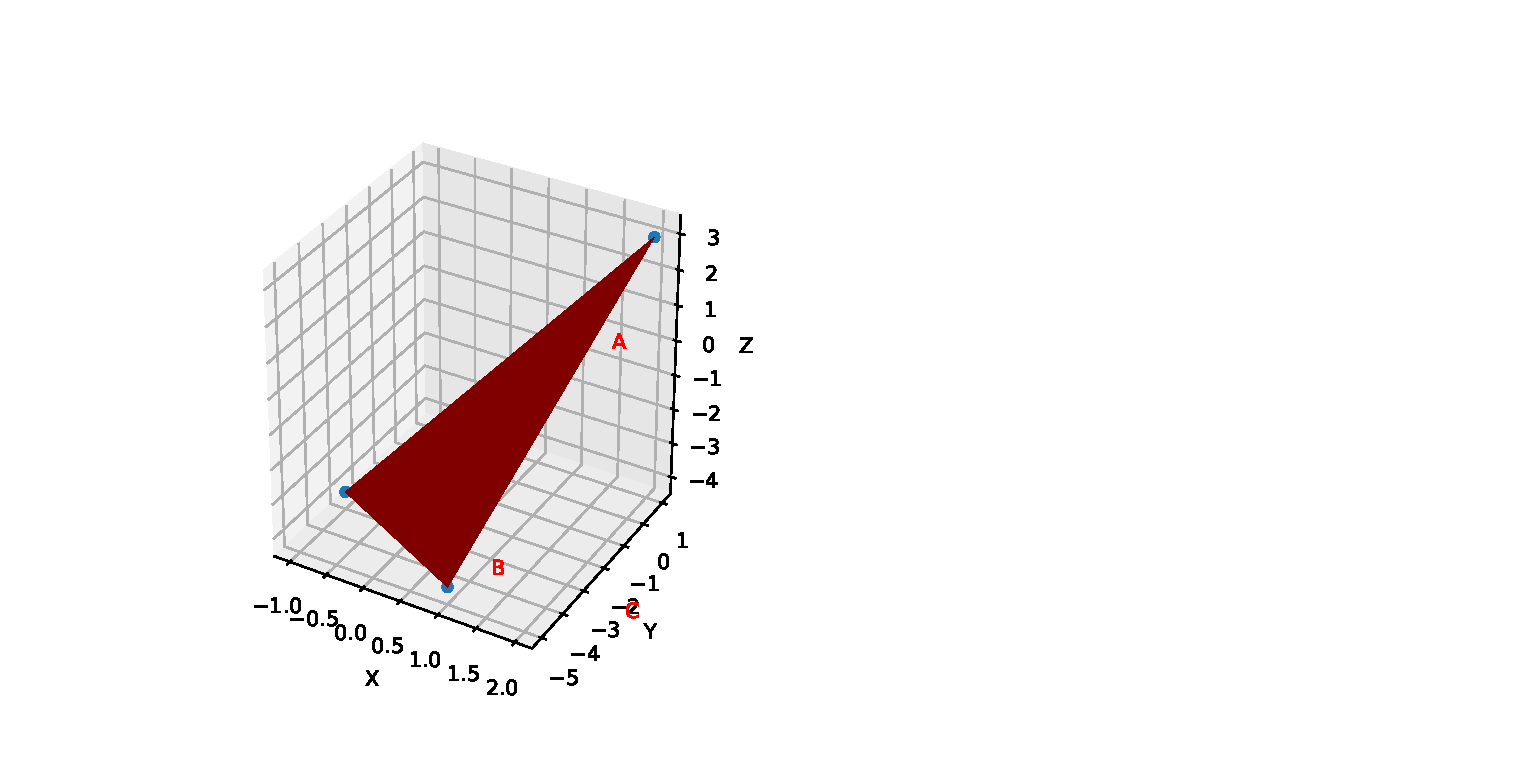
\includegraphics[width=\columnwidth]{./triangle/figs/triangle_3d.eps}
\caption{}
\label{fig:triangle_3d}
\end{figure}
%
From the figure, it appears that $\triangle ABC$ is right angled at $\vec{C}$.  Since 
\begin{align}
\brak{\vec{A}-\vec{C}}^T\brak{\vec{B}-\vec{C}}&=0
\end{align}
%
it is proved that the triangle is indeed right angled.
 \item Are the points 
\begin{align}
\vec{A} = \myvec{3\\6 \\9},
\vec{B} = \myvec{10\\20 \\30},
\vec{C} = \myvec{25\\ -41\\5},
\end{align}
%
the vertices of a right angled triangle?
%
\item A tower stands vertically on the ground.  From a point on the ground, which is 15m away from the foot of the tower, the angle of elevation of the top of the tower is found to be 60$\degree$.  Find the height of the tower.
%
\begin{figure}[!ht]
\includegraphics[width=\columnwidth]{./triangle/figs/Trig/pg1.eps}
\caption{}
\label{fig:trig_pg1}
\end{figure}
%
\\
\solution Fig. \ref{fig:trig_pg1} summarizes the problem. 
%
\begin{align}
h = b\tan\theta = 15\tan60\degree = 15\sqrt{3}
\end{align}
%
\item An electrician has to repair an electric fault pole of height 5m.  She needs to reach a point 1.3m below the top of the pole to undertake the repair work.  What should be the length of the ladder that she should use which, when inclined at an angle of 60$\degree$ to the horizontal, would enable her to reach the required position?  Also, how far from the foot of the pole should she place the foot of the ladder?
%
\begin{figure}[!ht]
\includegraphics[width=\columnwidth]{./triangle/figs/Trig/pg2.eps}
\caption{}
\label{fig:trig_pg2}
\end{figure}
%
\\
\solution Fig. \ref{fig:trig_pg2} summarizes the problem. The objective is to find $l$ and $b$.  From the figure,
%
if 
\begin{align}
\cot \theta &=\frac{1}{\tan \theta},
\\
h-x &= l\sin \theta = b\tan \theta
\\
\implies l &= \brak{h-x}\csc \theta = 3.7\csc60\degree 
\\
\text{and } b&=\brak{h-x}\cot\theta = 3.7 \cot \degree 
\end{align}
\item An observer 1.5m tall is 28.5m away from a chimney.  The angle of elevation of the top of the chimney from her eyes is 45$\degree$.  What is the height of the chimney?
%
%
\begin{figure}[!ht]
\includegraphics[width=\columnwidth]{./triangle/figs/Trig/pg3.eps}
\caption{}
\label{fig:trig_pg3}
\end{figure}
%
\\
\solution Fig. \ref{fig:trig_pg3} summarizes the problem. The objective is to find $h$.  From the figure,
%
\begin{align}
h-h_1 &=  b\tan \theta
\\
\implies h &= h_1+b\tan\theta 
\\
&= 1.5+28.5\tan45\degree 
\\
&= 30m
\end{align}
\item From a point $\vec{P}$ on the ground the angle of elevation of the top of a 10m tall building is 30$\degree$.  A flag is hoisted at the top of the building and the angle of elevation of the top of the flagstaff from $\vec{P}$ is $45\degree$.  Find the length of the flagstaff and the distance of the building from the point $\vec{P}$.
%
\begin{figure}[!ht]
\includegraphics[width=\columnwidth]{./triangle/figs/Trig/pg4.eps}
\caption{}
\label{fig:trig_pg4}
\end{figure}
%
\\
\solution Fig. \ref{fig:trig_pg4} summarizes the problem. The objective is to find $h_2$ and $b$ while $h_1$ is known.  From the figure, 
%
\begin{align}
h_1+h_2 &=  b\tan \theta_1
\\
h_1 &= b\tan \theta_2
\end{align}
%
This can be expressed as the matrix equation 
%
\begin{align}
\myvec{
\tan \theta_1 & -1
\\
\tan \theta_2 &0
}\myvec{b\\h_2}
= h_1\myvec{1\\1}
\end{align}
%
and solved.
\item The shadow of a tower standing on a level ground is found to be 40m longer when the Sun's altitude is 30$\degree$ than when it is $60\degree$.  Find the height of the tower.
%
\begin{figure}[!ht]
\includegraphics[width=\columnwidth]{./triangle/figs/Trig/pg5.eps}
\caption{}
\label{fig:trig_pg5}
\end{figure}
%
\\
\solution Fig. \ref{fig:trig_pg5} summarizes the problem. The objective is to find $h$.  from the figure,
%
\begin{align}
b_1 &= h\cot 60\degree
\\
b_2 &= h\cot 30\degree
\\
b_2-b_1 &= 40
\\
\implies h \brak{\cot 30\degree-\cot 60\degree}&= 40
\\
\text{or } h &= \frac{40}{\cot 30\degree-\cot 60\degree}
\end{align}
%
\item The angles of depression of the top and the bottom of an 8m tall building from the top of a multi-storeyed building are 30$\degree$ and 45$\degree$ respectively.  Find the height of the multi-storeyed building and the distance between the two buildings.
%
\begin{figure}[!ht]
\includegraphics[width=\columnwidth]{./triangle/figs/Trig/pg6.eps}
\caption{}
\label{fig:trig_pg6}
\end{figure}
%
\\
\solution Fig. \ref{fig:trig_pg6} summarizes the problem. The objective is to find $h_2$ and $b$.  From the figure, 
%
\begin{align}
h_2 &= b\tan \theta_2
\\
h_2-h_1 &= b\tan \theta_1
\end{align}
%
which can be expressed as
%
\begin{align}
\myvec{
 1 & -\tan\theta_2 
\\
 1 & -\tan\theta_1
}\myvec{h_2\\b}
= h_1\myvec{0\\1}
\end{align}
%
and solved.
\end{enumerate}
%
